\newcommand{\stage}[3]{\tikz{\node[shape=circle,draw,inner sep=1pt,fill=#1]{$#3_{#2}$};}}

\newcommand{\pos}[2]{\tikz{\node[shape=circle,draw,inner sep=1pt, fill=#1, minimum size = 0.6cm]{\scriptsize{$w_{#2}$}};}} 

\newcommand{\stages}[2]{\tikz{\node[shape=circle,draw,inner sep=1pt,fill=#1,minimum size=0.5cm]{\scriptsize{$v_{#2}$}};}} 

\newcommand{\leaf}{\tikz{\node[shape=circle,draw,inner sep=1.5pt,fill=white] {};}}
\newcommand\independent{\protect\mathpalette{\protect\independenT}{\perp}}
\def\independenT#1#2{\mathrel{\rlap{$#1#2$}\mkern2mu{#1#2}}}
\newcommand{\sage}[2]{\tikz{\node[shape=circle,draw,inner sep=1pt,minimum width = 0.6cm, fill=#1]{$v_{#2}$};}} 



\begin{figure}
    \centering
\scalebox{0.8}{
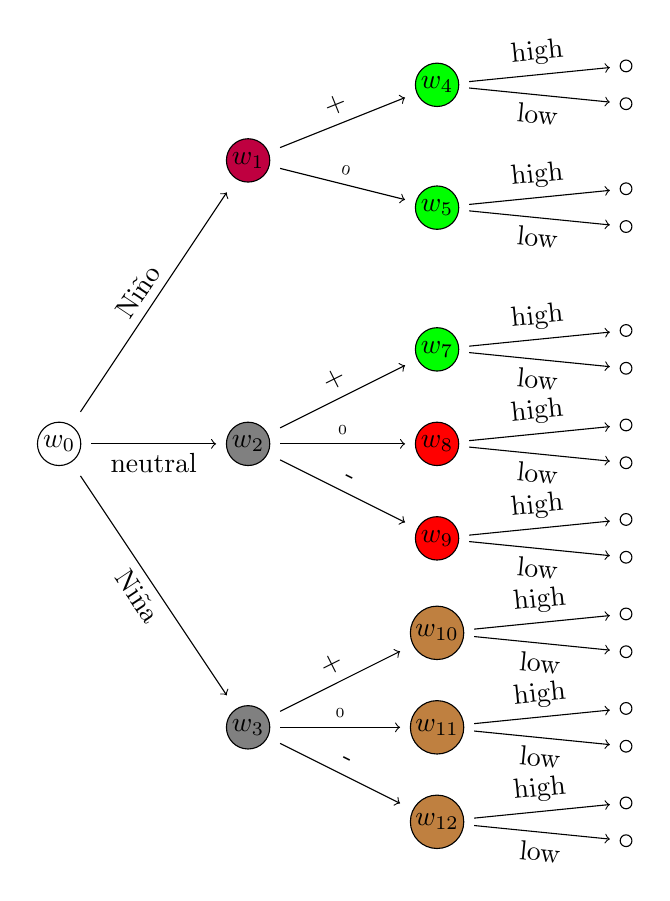
\begin{tikzpicture}
\newcommand{\xx}{2.4}
\newcommand{\yy}{1.2}
\node (w0) at (0*\xx,0*\yy) {\stage{white}{0}{w}};
\node (w1) at (1*\xx,3*\yy) {\stage{purple}{1}{w}};
\node (w2) at (1*\xx,0*\yy) {\stage{gray}{2}{w}};
\node (w3) at (1*\xx,-3*\yy) {\stage{gray}{3}{w}};
\node (w4) at (2*\xx,3.8*\yy) {\stage{green}{4}{w}};
\node (w5) at (2*\xx,2.5*\yy) {\stage{green}{5}{w}};
%\node (w6) at (2*\xx,1.5*\yy) {\stage{red}{6}{w}};
\node (w7) at (2*\xx,1*\yy) {\stage{green}{7}{w}};
\node (w8) at (2*\xx,0*\yy) {\stage{red}{8}{w}};
\node (w9) at (2*\xx,-1*\yy) {\stage{red}{9}{w}};
\node (w10) at (2*\xx,-2*\yy) {\stage{brown}{10}{w}};
\node (w11) at (2*\xx,-3*\yy) {\stage{brown}{11}{w}};
\node (w12) at (2*\xx,-4*\yy) {\stage{brown}{12}{w}};
\node (l1) at (3*\xx,4*\yy) {\leaf};
\node (l2) at (3*\xx,3.6*\yy) {\leaf};
\node (l3) at (3*\xx,2.7*\yy) {\leaf};
\node (l4) at (3*\xx,2.3*\yy) {\leaf};
\node (l5) at (3*\xx,1.2*\yy) {\leaf};
\node (l6) at (3*\xx,0.8*\yy) {\leaf};
%%%%%%%%%%%%%%%
\node (l7) at (3*\xx,0.2*\yy) {\leaf};
\node (l8) at (3*\xx,-0.2*\yy) {\leaf};
\node (l9) at (3*\xx,-0.8*\yy) {\leaf};
\node (l10) at (3*\xx,-1.2*\yy) {\leaf};
%%%%%%%%%%%
\node (l11) at (3*\xx,-1.8*\yy) {\leaf};
\node (l12) at (3*\xx,-2.2*\yy) {\leaf};
\node (l13) at (3*\xx,-2.8*\yy) {\leaf};
\node (l14) at (3*\xx,-3.2*\yy) {\leaf};
\node (l15) at (3*\xx,-3.8*\yy) {\leaf};
\node (l16) at (3*\xx,-4.2*\yy) {\leaf};
\draw[->] (w0) -- node [above, sloped] {Niño} (w1);
\draw[->] (w0) -- node [below, sloped] {neutral} (w2);
\draw[->] (w0) -- node [below, sloped] {Niña} (w3);
\draw[->] (w1) -- node [above, sloped] {+} (w4);
\draw[->] (w1) -- node [above, sloped] {\tiny $0$} (w5);
\draw[->] (w2) -- node [above, sloped] {+} (w7);
\draw[->] (w2) -- node [above, sloped] {\tiny $0$} (w8);
\draw[->] (w2) -- node [above, sloped] {-} (w9);
\draw[->] (w3) -- node [above, sloped] {+} (w10);
\draw[->] (w3) -- node [above, sloped] {\tiny $0$} (w11);
\draw[->] (w3) -- node [above, sloped] {-} (w12);
\draw[->] (w4)--node [above, sloped] {high} (l1); \draw[->] (w4)--node [below, sloped] {low}(l2);
\draw[->] (w5)--node [above, sloped] {high}(l3); \draw[->] (w5) --node [below, sloped] {low}(l4);
\draw[->] (w7)--node [above, sloped] {high}(l5); \draw[->] (w7) --node [below, sloped] {low}(l6);
\draw[->] (w8)--node [above, sloped] {high}(l7); \draw[->] (w8) --node [below, sloped]{low}(l8);
\draw[->] (w9)--node [above, sloped] {high}(l9); \draw[->] (w9) --node [below, sloped]{low}(l10);
\draw[->](w10)--node[above, sloped]{high}(l11);\draw[->](w10)--node[below,sloped]{low}(l12);
\draw[->](w11)--node [above, sloped]{high}(l13);\draw[->] (w11)--node[below,sloped]{low}(l14);
\draw[->](w12)--node[above, sloped]{high}(l15);\draw[->](w12)--node[below,sloped]{low}(l16);
%\node (tab) at (-2.2,-4) {
%\begin{tabular}{cc}
%     stage & $P($high AU$| \cdot)$ \\
%     \midrule
%    \textcolor{brown}{brown} & $0.833$ \\
%    \textcolor{red}{red} & $0.474$ \\
%     \textcolor{green}{green} & $0.222$ \\   
%\end{tabular}
%};
\end{tikzpicture}
}
  %  \caption{Staged tree estimated with the BHC algorithm for the 
  %  ENSO-IOD-AU example and 
  %  estimated conditional probabilities for 
  %  high AU in the three recovered stages.}
    \label{fig:enso}
\end{figure}
